\section{ReCapture Design}\label{sec:design}
The ultimate goal of ReCapture is to give a researcher or developer the capability to run a large scale evaluation about smartphones automatically. Therefore, the design of ReCapture needs the following criterion.
\begin{itemize}
\item Generalness. ReCapture should provide the simple and unified interface for the researches or developers that whatever they want to evaluate on this testbed, they can use the same tool and the same APIs.
\item Flexibility. It requires ReCapture to give the chance for the testbed's input, execution pattern and performance monitoring.
\end{itemize}

\subsection{Core System}
Fig.~\ref{fig:big} shows the big picture of ReCapture. As we can see, we have a central master to organize and schedule testbed and the mobile devices are the testbed to automatically execute the activity log. The central master will load the existing activity log for each device, once the smartphone receive the log activity completely it starts executing the activity script one by one. After the smartphone pull an app in the foreground screen, the central master will be informed which the central master will start sending screen actions to the corresponding smartphone. The screen action script is flexible and can be defined by the developers themselves.

\begin{figure}
\centering
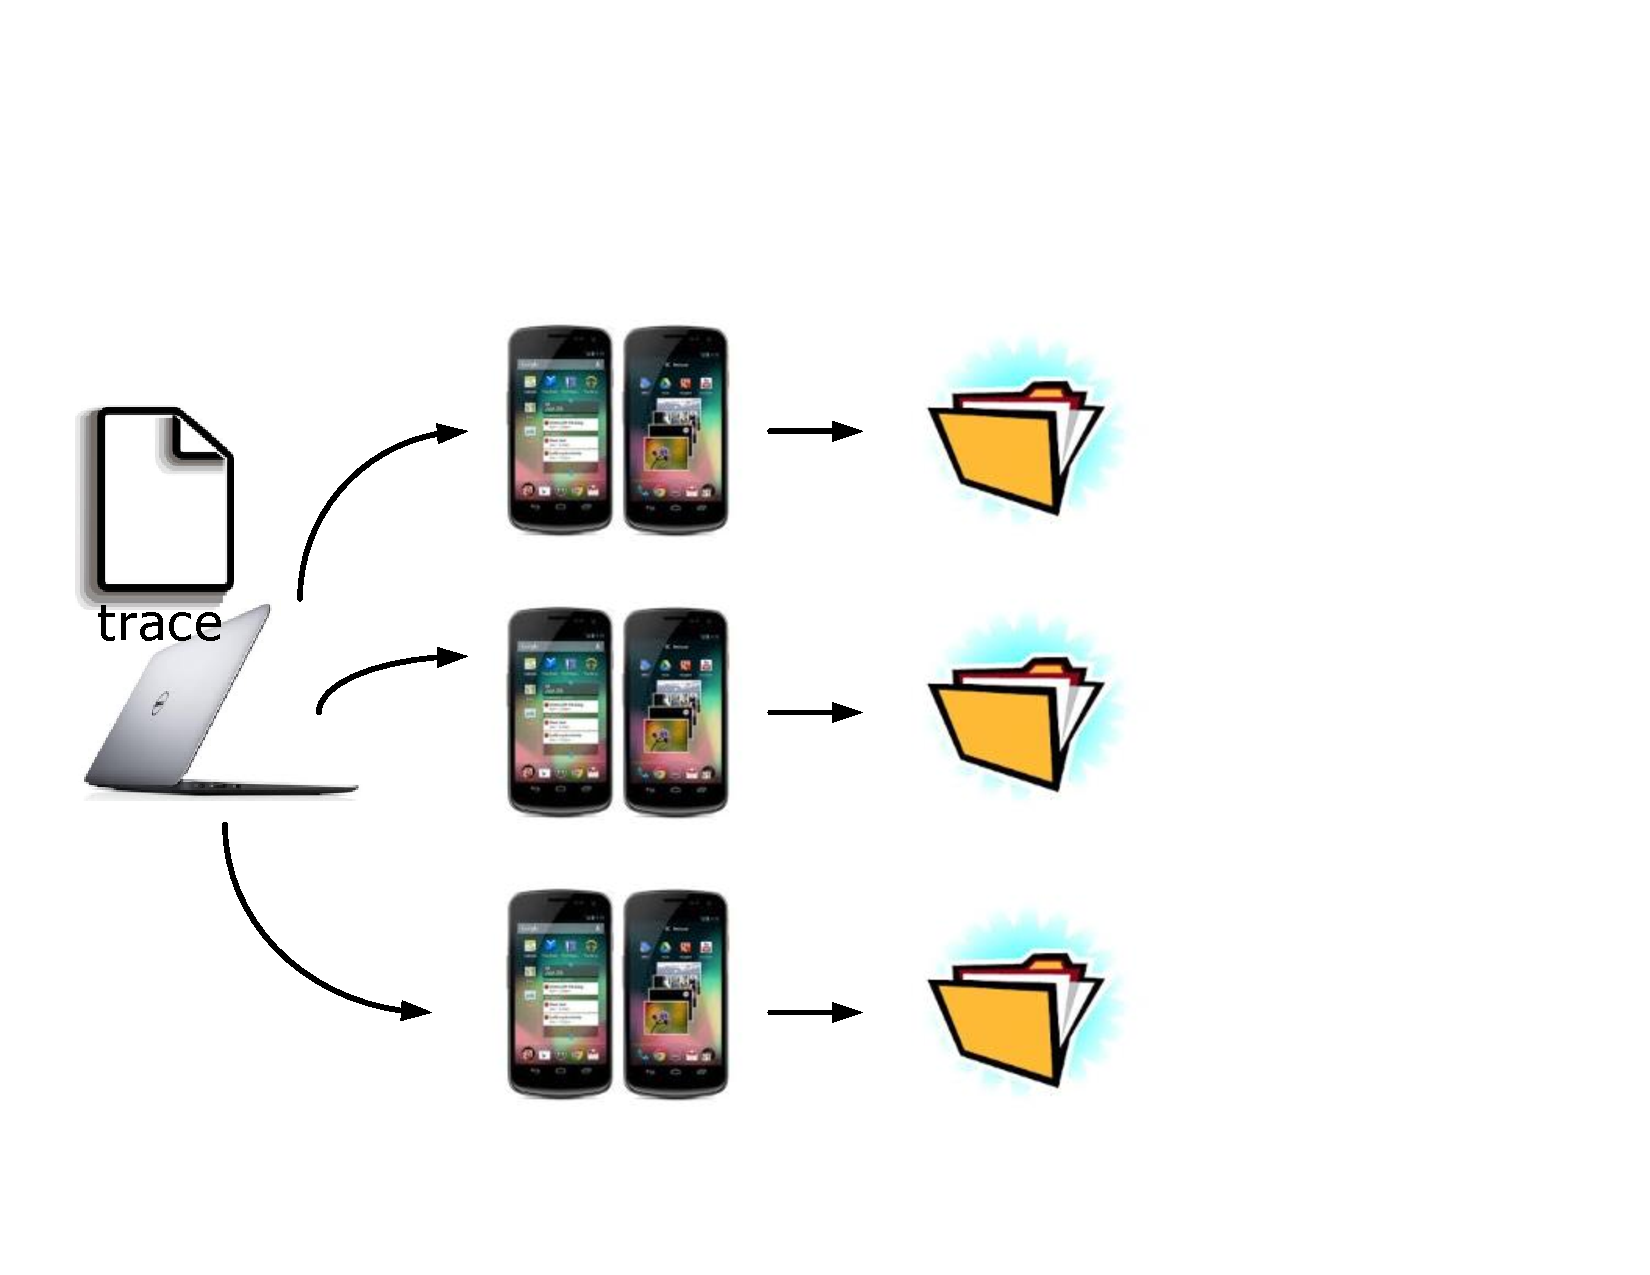
\includegraphics[width=0.45\textwidth]{figures/big-picture.pdf}
\caption{The Big Picture of ReCapture}
\label{fig:big}
\end{figure}

The system architecture is shown in Fig.~\ref{fig:sys}. As is shown, two separate parts are in the system's core architecture: device side and central master side. In the device side, two lightweight components support the runtime environment of the testbed. One is the \emph{scheduler} and the other is \emph{app trigger}. The scheduler takes the activity log (or data trace) received from the central master, then it arranges the execution sequence based on the activity log. For each of the activity event, it starts an app trigger which brings the dedicated app into the screen front. As soon as the the the app is running, the scheduler will send a message to the central master, which will start issuing the screen actions to the device.

Besides the major components, the performance monitor module is presented as a plugin which is flexible to be added and removed. For example, if the developer is interested in the energy consumption of the operating system, he can plugin the energy profiling module into this component. We do not provide identical performance monitoring module inside the ReCapture's framework because 1) we do not want to restrict the extendibility of the system by hard-code everything; 2) we do not want to waste the operating system's resource if the developer is not interested in some monitor like dynamic CPU cost.

On the other hand, the central master have three important modules: synchronization, touch modeling and touch injection. The synchronization module is used to listen the scheduler's commands so that the correct screen actions can be issued. In fact, different app has different usage pattern, so it is important to differentiate among them and model various screen events. Then the screen modeling is the place to model an app's usage action. Normally, a developer can define a series screen actions, this module will go ahead and load the scripts. After the screen action is defined, the touch injector will send the screen actions to the device continuously until the next activity event comes.

\begin{figure}
\centering
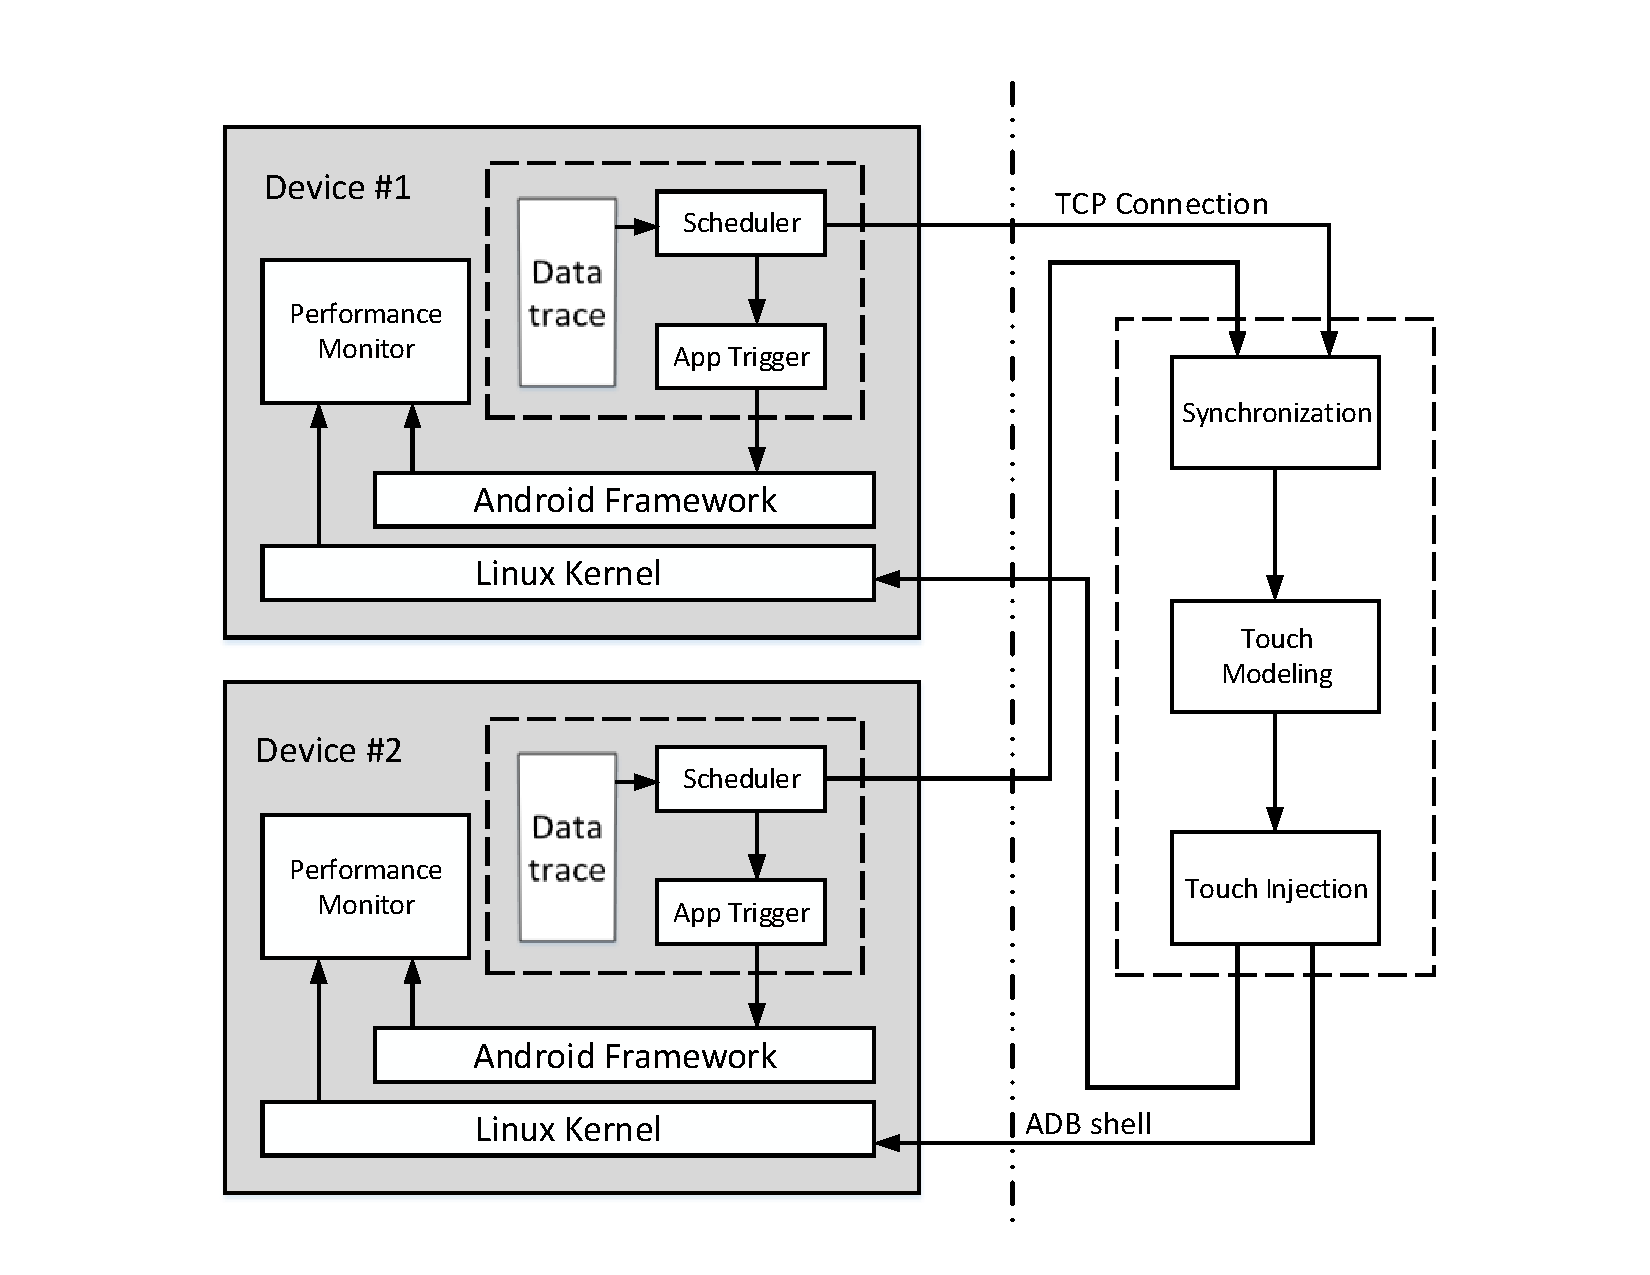
\includegraphics[width=0.45\textwidth]{figures/sys-arch.pdf}
\caption{ReCapture System Architecture}
\label{fig:sys}
\end{figure}

\subsection{Traces and Screen Operations}
As we have discussed, the activity log comes from the existing trace. For example, the \emph{Livelab} data set from Rice University has an app usage trace of $25$ users. The critical information of the data trace includes package name, start time and duration. This three tuple gives the exact running period of an activity event. The package name identify which app and its UI needs to bring to the screen front; the start time gives the relative sequential information of different activity events, which actually is not as important as the package name and the duration; finally the duration specifies how long the app will be use, then the central master will continue issue enough screen actions within the usage period. 

Since the app start timestamp is not as important as the rest two factors, we usually do not need to contain the timestamp information but we require the order of the activity events in the log is first happen first schedule. Then a configurable gap between activity events will be inserted, replacing the original idle period in the data trace. We change the trace in this way simply because we need to shrink the execution time. For instance, the Livelab data trace lasts about one year, but we cannot wait for a year. After we analyze the data set, we find most of the time is idle, so it is safe to replace the large amount of idel period with a fixed gap between activity events.

A sample process is shown in Fig.~\ref{fig:big2}. The central master will take the trace and assign the activity event to different device in time sequence. Thus, each device should have a timeline to trigger the activity event in the smartphone. All devices trigger its own activity event after receiving the activity event from the central master, and the trigger is independent among all devices.

\begin{figure}
\centering
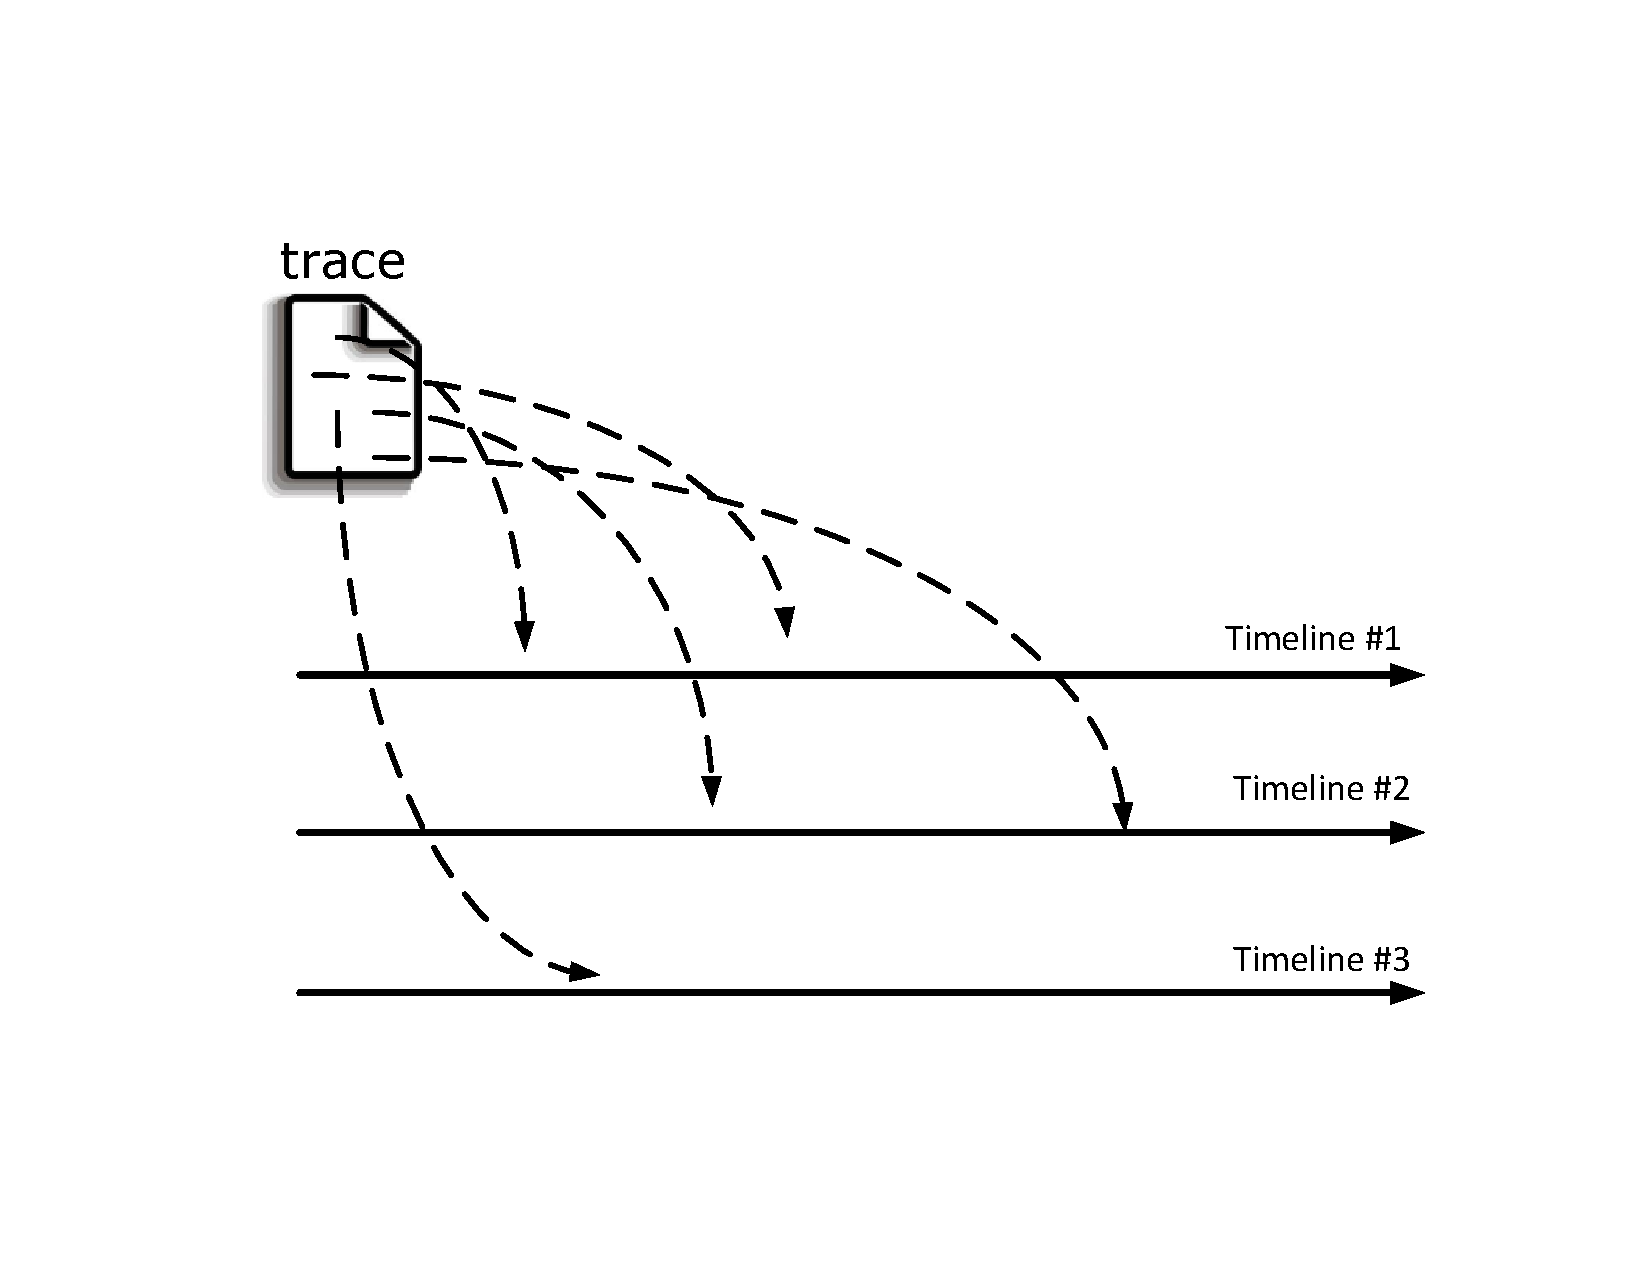
\includegraphics[width=0.45\textwidth]{figures/big-picture2.pdf}
\caption{A sample trace assignment}
\label{fig:big2}
\end{figure}

\subsection{Scalability}
Another important feature in the ReCapture framework is the scalability, which should scale up as many devices as possible at the same time. The reason is obvious that the more devices running simultaneously, the more data we will collect.

Suppose we have unlimited number of physical devices, the scalability is easy to control because we just need to open more USB ports for the extra devices. Unfortunately, the reality is not so convenient in two fold: 1) the number of USB port is not infinite, but our experiment may requires thousands of devices running together; 2) we may only afford less than $10$ devices at a time. Therefore, we need to use an alternative approach to reach the scalability.

Virtualization seems to be the only solution to make the scalability possible and linearly scale up. If we virtualize the physical environment of the smartphone, we may be able to scale $5$ times or more. Existing works have explored the possibility relatively well, so we do not spend too much effort in the virtualization part or scalability issue here.
